%% LyX 2.0.6 created this file.  For more info, see http://www.lyx.org/.
%% Do not edit unless you really know what you are doing.
\documentclass[12pt,oneside,english]{amsart}
\usepackage{ae,aecompl}
\usepackage[T1]{fontenc}
\usepackage[latin9]{inputenc}
\pagestyle{plain}
\usepackage{amsthm}
\usepackage{amssymb}
\usepackage{graphicx}

\makeatletter
%%%%%%%%%%%%%%%%%%%%%%%%%%%%%% Textclass specific LaTeX commands.
\numberwithin{equation}{section}
\numberwithin{figure}{section}

%%%%%%%%%%%%%%%%%%%%%%%%%%%%%% User specified LaTeX commands.
\usepackage{graphicx}
\usepackage{amsfonts}

\makeatother

\usepackage{babel}
\begin{document}

\title{Expected Utility and Risk Aversion}


\author{Michael Peters}


\date{\today{}}

\maketitle

\section{Introduction}

This reading describes how people's aversion to risk affects the decisions
they make about investment. Basically, the concepts used to do this
analysis emerge naturally when people have expected utility preferences,
but not otherwise. So, it illustrates one important way that expected
utility is applied. 

This analysis also makes it possible to illustrate how to do \emph{comparative
statics}. Comparative statics typically involve calculations designed
to show the direction in which changes in the environment move peoples'
optimal decisions. Convincing comparative static results are ones
that hold even if you only impose weak restrictions on preferences.
So, for instance, to explain how an increase in price affects a buyer's
demand when he or she has Cobb-Douglas preferences is not very convincing
because Cobb Douglas preferences are a very special case. In fact,
as we have already shown, an (uncompensated) increase in price will
only reduce demand under very special conditions. That is why the
method for doing comparative statics tend to be a little more sophisticated,
and the questions asked tend not to be the most obvious ones. 


\subsection{Lotteries with a Continuum of Outcomes}

In portfolio theory, outcomes are all monetary. We looked at monetary
lotteries in some of the example above. Yet it doesn't make sense
when thinking about stocks or bonds to restrict to only three or four
outcomes, there are really an infinity of possible outcomes. The way
to think about this is to think of the set of potential outcomes $\mathcal{X}$
as an interval of $\mathbb{R}$. Of course, we can't assign a positive
probability to each of these outcomes the way we have so far. So instead
we describe a lottery as a \emph{probability distribution function,}
$F(x)$ that takes each possible value $x$ in the set of \emph{potential}
outcomes and gives the probability that the \emph{actual} outcome
is less than or equal to $x$.

We could actually describe the lotteries we have considered so far
this way. For example, in the last chapter we thought about lotteries
with three outcomes, in particular, the outcomes were$\{1000,500,0\}$,
where each of these outcomes is supposed to be a monetary outcome.
We assigned probability $p_{1}$ to the first outcomes, $p_{2}$ to
the second and $p_{3}=1-p_{1}-p_{2}$ to the third. 

Suppose we think of $\mathcal{X}=[-100,+2000]$ as the set of possible
outcomes. Then the following diagram shows you what the corresponding
probability distribution function looks like for this lottery. The
function $F(x)$ starts out at 0 when $x$ is equal to $-100$ which
is the lowest possible monetary payoff.\\
\begin{figure}
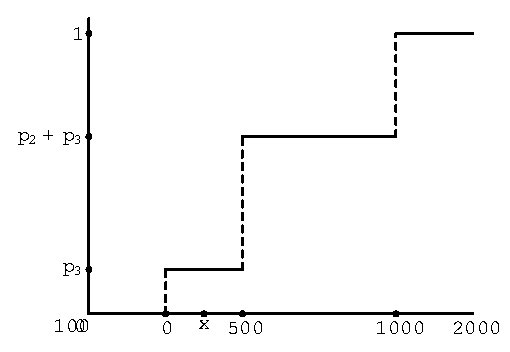
\includegraphics{risk_aversion_fig2}
\end{figure}
For every value of $x$ between $-100$ and $0$ the probability that
the outcome of the lottery is less than or equal to these values is
constantly zero. However, the probability that the outcome of the
lottery is less than or equal to $0$ is exactly equal to the probability
that $0$ occurs, in other words, $p_{3}$, the probability that we
have been assigning to the worst outcome. As the monetary payoff travels
between $0$ and $500$, say a value like $x$ in the diagram, the
probability that the outcome is less than or equal to $x$ is then
constant at $p_{3}$. Suddenly it jumps up to $p_{2}+p_{3}$ when
$x$ is $500$, and so on, until it reaches 1 and stays there after
$x$ is $1000$.

The previous chapter showed how the independence axiom makes it possible
to compare different lotteries by computing the \emph{expected utility}
associated with those lotteries. The expected utility associated with
the lottery $\{p_{1},p_{2},p_{3}\}$ for example, is given by
\[
p_{1}u(1000)+p_{2}u(500)+p_{3}u(0)
\]
 The lottery $\{p_{1},p_{2},p_{3}\}$ is the same as the probability
distribution described in the Figure above.

Now suppose that we want to describe a lottery with an infinite number
of outcomes, for example, a share that has a return that could be
anything between $-100$ and $2000$. We can't describe such a lottery
by assigning probabilities to each possible outcome in this case.
There are just too many of them. We could, however, still describe
the lottery by giving the probability distribution function associated
with it. An infinite lottery might have a probability distribution
that looked like the one in the next figure.

\begin{figure}
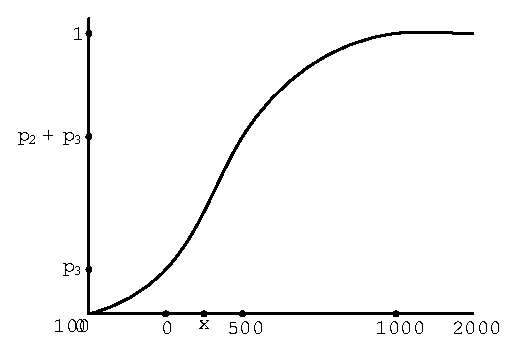
\includegraphics{risk_aversion_fig3}
\end{figure}
This lottery (i.e., the probability distribution function associated
with this lottery) has the same values at $0$, $500$, and $1000$
as the previous lottery - $p_{3},$ $p_{2}+p_{3}$, and $1$. However,
at a point like $x$, the probability that the outcome in this lottery
is less than or equal to $x$ is strictly higher than $p_{3}$ which
was its value in the previous lottery.

The expected utility theorem suggests that if the independence axiom
holds for compound lotteries described as distribution functions,
then we should be able to assign a utility value to \emph{all} the
outcomes between $-100$ and $2000$. Then if we could somehow multiply
these utility values by something like probabilities associated with
each outcome we would have a single utility value for the lottery.
The way to do this is to \emph{integrate} the utility values multiplied
by the amount by which the probability distribution function increases
at each possible outcome. This expression looks like
\[
\int_{-100}^{2000}u(x)dF(x)
\]
where $dF(x)$ means the \emph{change} in the probability distribution
function. For a lottery like the first of the two above, $dF$ is
equal to zero at every point except for the three special outcomes,
$0$, $500$, and $1000$. Then, $dF$ takes the values $p_{3}$,
$p_{2}$ and $p_{1}$ respectively. Then if we add up by integrating
as above we just get the sum
\[
p_{1}u(1000)+p_{2}u(500)+p_{3}u(0)
\]


In a case like the second lottery, $dF$ is the \emph{derivative}
of the probability distribution (sometimes called its density). In
that case you would write $dF$ as $F^{\prime}(x)dx$ where $F^{\prime}(x)=\frac{dF(x)}{dx}$.
That is the formulation you have probably seen before.

As an example, one special probability distribution function is the
\emph{uniform} distribution function. The idea behind it is that every
possible outcome is equally likely. So if you take a point midway
through the set of outcomes, i.e. 1050, then the probability the outcome
is less than or equal to 1050 should be equal to $\frac{1}{2}$. The
probability distribution that does this is
\[
F(x)=\frac{x-(-100)}{2000-(-100)}
\]
The expected utility associated with this lottery is
\[
\frac{1}{2100}\int u(x)dx
\]
 because of the fact that $F^{\prime}(x)=\frac{1}{2100}$. Then using
your high school algebra, the expected utility associated with the
lottery whose probability distribution function is uniform is just
the ratio of the area under the utility function between $-100$ and
$2000$, to the area in the rectangle whose sides have length 1 and
2100.


\subsection{Risk Aversion}

As described above, the independence axiom implies that there is a
\emph{utility for wealth} function that people use to evaluate lotteries.
One reasonable question to ask is whether we could guess something
about the shape of this function from other properties of behavior.
For example, the St. Petersberg bet that we discussed in the last
chapter has an infinite expected value, but no one would pay an infinite
amount to engage in the bet. 

An even simpler example might be the following - I propose a new grading
scheme for the exam. You can choose either of the following options
- either take the mark you get, or I will flip a coin - heads I raise
your mark by 10 points, tails I lower your mark by 10 points. Your
expected grade is the same under either scheme. You probably wouldn't
want the second scheme because it is risky\emph{.} An A grade could
turn into a B, a pass could turn into a fail (or conversely).

The second grading scheme involves what is called a \emph{fair} gamble
in the sense that the expected gain to you of taking the bet is exactly
zero. It seems plausible that most people simply wouldn't be interested
in taking a fair bet.%
\footnote{However, it should be added that the bets that people take in a casino
are not fair. For example, if you fed coins into a slot machine for
the rest of your life you would lose a lot of money. This doesn't
seem to stop people from going to casinos.%
}%
\footnote{The lotteries that you buy into at the corner store (like the Lotto
6-49) represent a strange variant on what happens in casinos. The
way the lotteries work is roughly as follows - the lottery sells tickets.
From the total revenue they earn by ticket sales, they take out a
big chunk to cover operating costs and to give themselves some profit.
The rest is put in a pool. A number is then drawn randomly by dropping
balls from an urn (or some other method that is independent of the
number of tickets). If one or more people has the winning number they
split all the money in the pool. The interesting event occurs when
no one has the ticket. Then, when the lottery is run the next period,
a portion of ticket sales is added to the pool which already contains
the pool from the last lottery. If no one wins for a long time, the
pool can become so large that the lottery ticket will be a more than
fair bet. For example, as this is written the chance of winning the
6-49 is about 1 in 18 million, but the current pool of money to be
won is about 40 million. So the lottery ticket appears to have an
expected value of a little over \$2. It only costs \$2 to buy a ticket.
So it appears that everyone should buy a ticket. Many people do, leading
to enormous revenues and profits for the lottery corporation. This
is a bit misleading because the odds of winning are independent of
the number of bidders. That means that if many people bid, more than
one person is likely to have a winning ticket. The average payout
to a winner will be considerably smaller than \$40 million for this
reason, which makes the expected value of the ticket smaller than
\$2.%
} This kind of behavior does have some implications for the shape of
the utility function. You can what the implications are in the next
figure.\\
\begin{figure}
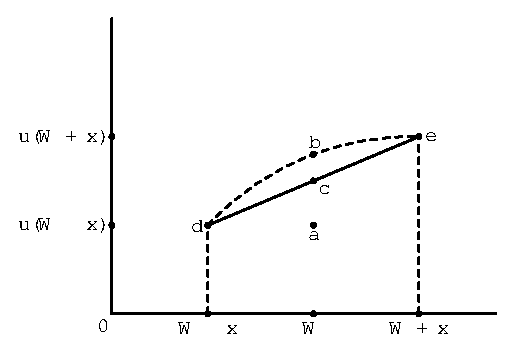
\includegraphics{risk_aversion_fig4}
\end{figure}
Suppose our consumer has some initial level of wealth $W$. A fair
bet is one whose expected return is zero. One example would be a bet
that pays $x$ with probability $\frac{1}{2}$, but which costs you
$x$ with the same probability. Doing nothing leaves you with $W$
for sure. The independence axiom implies that there is a utility level
$u(W)$ associated with this outcome. The outcomes $W-x$ and $W+x$
also have associated utility values $u(W-x)$ and $u(W+x)$. These
are marked in the diagram. The expected utility of the lottery we
just described is then
\[
\frac{1}{2}u(W-x)+\frac{1}{2}u(W+x)
\]
In the diagram, this utility level is the distance from the point
$W$ on the horizontal axis up to the point $c$ in the diagram.%
\footnote{To see this observe that the vertical distance between the points
d and e is $u(W+x)-u(W-x)$. By similar triangles, the ratio of the
vertical distance between a and c (call it $|c-a|$) to $u(W+x)-u(W-x)$
is the same as the ratio of the horizontal distance between a and
d to $W+x-(W-x)$. This latter ratio is equal to $\frac{1}{2}$. Therefore
\[
|c-a|=\frac{1}{2}(u(W+x)-u(W-x))
\]
Now adding $u(W-x)$ to both sides gives 
\[
|c-d|+u(W-x)=\frac{1}{2}u(W-x)+\frac{1}{2}u(W+x)
\]
%
} The assertion that our consumer would rather not engage in this bet
means that the utility value of $W$ (for sure) must be above c at
a point like b. Since this preference not to take fair bets is likely
to be true no matter what $x$ is and no matter what $W$ is, means
that the utility for wealth function must lie everywhere above the
line segment from d to e. In other words, the utility for wealth function
must be concave.


\subsection{Measuring Aversion to Risk}

Stocks and bonds are more complex than lotteries because the monetary
outcomes usually aren't fair. Most traded stocks for example have
a positive expected return. The thing that makes stock trading interesting
is that it involves considerable risk. Whether or not an investor
will want an initial public offering of some stock depends partly
on the risk characteristics of the stock, and partly on the investors
own attitudes toward risk. The economics literature has suggested
some interesting ways of separating these two things.

Let $F$ be the probability distribution over outcomes that is associated
with some lottery. The expected payoff associated with the lottery
is
\[
\mathbb{E}x\mathbb{=}\int xdF(x)
\]
 where $dF(x)$ depends on the nature of the lottery as discussed
above. Lets assume for now that the probability distribution function
$F$ has a density so that we can write the expected payoff (and all
the expected utility calculations) using the better known manner
\[
\mathbb{E}x=\int xF^{\prime}(x)dx
\]
 

Let $W$ be any level of wealth. Lets try to calculate the maximum
amount our consumer would be willing to pay to play this lottery $F$.
Using the independence axiom we would find this price $p$ by solving
\[
u\left(W\right)=\int u\left(W-p+x\right)F^{\prime}\left(x\right)dx
\]
 It is going to tough to solve this exactly without more precise information
about $u$ so lets solve it 'approximately'. 

First take a second order Taylor approximation to the utility function
inside the integral sign on the right hand side of the equation. A
first order Taylor approximation won't work very well here because
it only gives a good approximation when $x$ is small. However, there
will typically be some risk that $x$ could be quite large, so some
correction for the curvature in $u$ will help. The second order approximation
is given by
\[
\int\left\{ u\left(W\right)+u^{\prime}\left(W\right)(x-p)+u^{\prime\prime}\left(W\right)\frac{(x-p)^{2}}{2}\right\} F^{\prime}\left(x\right)dx
\]
 If this is a good approximation, then it is approximately equal to
$U(W)$ when we choose the right $p$, so simplify the equation
\[
\int\left\{ u\left(W\right)+u^{\prime}\left(W\right)(x-p)+u^{\prime\prime}\left(W\right)\frac{(x-p)^{2}}{2}\right\} F^{\prime}\left(x\right)dx=u(W)
\]
to get
\[
u^{\prime}\left(W\right)\int(x-p)F'(x)dx+u^{\prime\prime}\left(W\right)\int\frac{(x-p)^{2}}{2}F^{\prime}\left(x\right)dx=0
\]
or
\[
p=\int xF^{\prime}(x)dx+\frac{u^{\prime\prime}(w)}{u^{\prime}(w)}\int\frac{(x-p)^{2}}{2}F^{\prime}(x)dx
\]
The second term in this expression has a $u^{\prime\prime}(w)$ which
is negative if the utility for wealth function is concave. So the
expression says that the maximum amount the consumer will be willing
to pay for the lottery is equal to its mean return less a term consisting
of two parts. One part is the integral which is related to the variance
of the lottery or the degree to which it is spread out and unpredictable.
The other part depends only on the consumer's utility for wealth function.
The larger in absolute value is the ratio $\frac{u^{\prime\prime}(w)}{u^{\prime}(w)}$,
the less the consumer will be willing to pay. 

This particular decomposition has proved to be very useful in thinking
about portfolio theory. The term
\[
-\frac{u^{\prime\prime}\left(W\right)}{u^{\prime}\left(W\right)}
\]
 is referred to as the Arrow-Pratt measure of absolute risk aversion. 

We will shortly see how this measure can be used to get some insight
into the way that investment decisions work. For the moment, the main
thing to note is that the Arrow-Pratt measure is a conceptual device
that emerges with the help of the expected utility theorem. One natural
assumption would seem to be that the risk premium that a consumer
would be willing to pay to avoid risk would be lower if the consumer
were more wealthy. The formulation so far shows exactly how to formalize
this idea - the function $-\frac{u^{\prime\prime}\left(W\right)}{u^{\prime}\left(W\right)}$
should be a decreasing function. We will come back to this idea momentarily. 


\subsection{The Portfolio Problem}

A fairly simple version of the portfolio problem can be studied by
assuming that there are exactly two different securities that an investor
can buy. A \emph{security} is a lottery. The consequences of the lottery
are possible rates of return on investment. If the consequence of
the lottery is a rate of return $s$, then the security pays $1+s$
dollars tomorrow for each dollar that is invested in the lottery today.
In the problem that we are going to analyze, one of the two securities
is safe in the sense that the lottery that produces the rate of return
gives a rate of return of zero for sure. So, each dollar invested
today gives back exactly one dollar tomorrow, no more and no less.
There is also a risky security where the probability distribution
function for the random rate of return is $F$.\ Sometimes this rate
of return will be positive and the security will pay back more than
one dollar for each dollar invested. Other times the rate of return
will actually be negative, and a dollar invested will return less
than one dollar tomorrow. 

The investor has $w$ dollars to invest in these two securities. His
\emph{ex post} income (i.e., his income tomorrow after the rate of
return on the lottery is realized) when he invests $i_{s}$ in the
safe security and $i_{r}$ in the risky security, is given by
\[
i_{s}+i_{r}\left(1+s\right)
\]


A pair $\left(i_{s},i_{r}\right)$ is called a \emph{portfolio}. Each
portfolio generates a different lottery over monetary outcomes. Then
relying on the independence axiom, we can invoke the expected utility
theorem and conclude that there is a utility for wealth function $u$
such that one portfolio (and its associated lottery) $\left(i_{s},i_{r}\right)$
is preferred to another $\left(i_{s}^{\prime},i_{r}^{\prime}\right)$
if
\[
\int u\left(i_{s}+i_{r}\left(1+s\right)\right)F^{\prime}\left(s\right)ds\geq
\]
\[
\int u\left(i_{s}^{\prime}+i_{r}^{\prime}\left(1+s\right)\right)F^{\prime}\left(s\right)ds.
\]


If that is true, then the investor should choose the portfolio that
maximizes
\[
\int u\left(i_{s}+i_{r}\left(1+s\right)\right)F^{\prime}\left(s\right)ds
\]
 subject to the constraints that
\[
i_{s}+i_{r}\leq W
\]
\[
i_{r}\geq0
\]
\[
i_{s}\geq0
\]


We could solve this using Lagrangian methods, recalling that before
you do so, you need to tease out some properties of the solution in
order to guess which constraints are likely to be important. To see
a way to do this, simply imagine that the integral above is just a
particular function
\[
U\left(i_{s},i_{r}\right)\equiv
\]
\[
\int u\left(i_{s}+i_{r}\left(1+s\right)\right)F^{\prime}\left(s\right)ds
\]
 and that the first constraint above is just a budget constraint where
the prices of both securities are just equal to $1$. So, we should
be able to find the optimal portfolio by finding the highest indifference
curve that touches the budget constraint, as the indifference curve
$II$ does in Figure $1$.
\begin{figure}
\centering{} 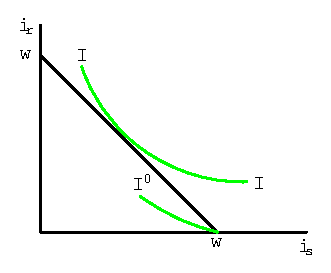
\includegraphics[
height=1.6302in,
width=2.0263in
]{risk_aversion_fig1.eps}
\end{figure}


The slope of the indifference curve is given by the marginal utility
of the good on the horizontal axis (i.e., $i_{s}$) divided by the
marginal utility associated with the good on the vertical axis (i.e.,
$i_{r}$). Differentiating gives
\[
-\frac{\frac{\partial U\left(i_{s},i_{r}\right)}{\partial i_{s}}}{\frac{\partial U\left(i_{s},i_{r}\right)}{\partial i_{r}}}=
\]
\[
-\frac{\int u^{\prime}\left(i_{s}+i_{r}\left(1+s\right)\right)F^{\prime}\left(s\right)ds}{\int u^{\prime}\left(i_{s}+i_{r}\left(1+s\right)\right)\left(1+s\right)F^{\prime}\left(s\right)ds}
\]


Now, following our usual procedure, we can try to check the conditions
under which we might find a solution at the corner where all wealth
is invested in the riskless asset. This would occur if the indifference
curve happened to be steeper than the budget line. So, let's evaluate
the slope of the indifference curve at the bundle $\left(w,0\right)$.
Substituting into the formula above gives
\[
-\frac{\int u^{\prime}\left(w\right)F^{\prime}\left(s\right)ds}{\int u^{\prime}\left(w\right)\left(1+s\right)F^{\prime}\left(s\right)ds}=
\]
\[
-\frac{1}{1+\int sF^{\prime}\left(s\right)ds}
\]
 This means that whether or not the investor optimally invests in
the risky asset depends entirely on $\int sF^{\prime}\left(s\right)ds$.
If this is positive, the (absolute value of the) slope of the indifference
curve is smaller than $1$ and the tangency has to occur somewhere
up the budget line to the left of $\left(w,0\right)$. On the other
hand, if the mean value of $s$ is less than zero, then the indifference
curve will be steeper than the budget line, and the optimal solution
will be at the corner of the budget set. 

This is called the \emph{diversification theorem}. If there is a risky
asset whose expected return exceeds the expected return on the safe
asset, then the optimal portfolio will always involve some investment
in the risky asset. 


\subsubsection{Comparative Statics and Wealth}

We might assume that wealthy people invest more in risky assets. This
assertion seems that it must be true. Surprisingly, this is not always
the case. It is difficult to see why this might be by using intuition
alone. As I have often mentioned, this is when mathematics can be
very useful. Intuition is rarely wrong: it just doesn't give the whole
story. Math can often help you think out the parts that you tend to
gloss over when you think intuitively. Often the biggest insights
in economics come by understanding the complexities that intuition
can't see. 

The problem that is discussed in this section also provides an opportunity
to see the way that comparative statics is often done in applications.
We are interested in what the effect of a change in wealth $w$ will
be on the optimal portfolio. One way to figure this out is to try
to find out how a change in wealth will affect the position of the
tangency between the indifference curve and budget line. To see how
this line of argument works, start by substituting the fact that $i_{s}=w-i_{r}$
into the tangency condition to get
\[
\frac{\int u^{\prime}\left(w-i_{r}+i_{r}\left(1+s\right)\right)F^{\prime}\left(s\right)ds}{\int u^{\prime}\left(w-i_{r}+i_{r}\left(1+s\right)\right)\left(1+s\right)F^{\prime}\left(s\right)ds}=1
\]
 Simplifying the arguments of the functions gives
\[
\frac{\int u^{\prime}\left(w+i_{r}s\right)F^{\prime}\left(s\right)ds}{\int u^{\prime}\left(w+i_{r}s\right)\left(1+s\right)F^{\prime}\left(s\right)ds}=1
\]
 Multiplying both sides by the denominator on the left gives
\[
\int u^{\prime}\left(w+i_{r}s\right)F^{\prime}\left(s\right)ds-\int u^{\prime}\left(w+i_{r}s\right)\left(1+s\right)F^{\prime}\left(s\right)ds=0
\]
 Canceling the common terms gives the equation
\begin{equation}
\int u^{\prime}\left(w+i_{r}s\right)sF^{\prime}\left(s\right)ds=0\label{FOC}
\end{equation}


The trick at this point is to assume that $i_{r}$ is actually a function
of $w$ that adjusts in such a way that the equation above is always
satisfied. Then, in fact,
\[
\int u^{\prime}\left(w+i_{r}\left[w\right]s\right)sF^{\prime}\left(s\right)ds\equiv0
\]
 Since this holds uniformly under this definition, we can differentiate
both sides of the expression with respect to $w$ and the derivatives
will also be equal. In other words
\[
\int u^{\prime\prime}\left(w+i_{r}\left[w\right]s\right)sF^{\prime}\left(s\right)ds+\int u^{\prime\prime}\left(w+i_{r}\left[w\right]s\right)\frac{di_{r}\left[w\right]}{dw}s^{2}F^{\prime}\left(s\right)ds=0
\]
 Solving for the derivative gives
\[
\frac{di_{r}\left[w\right]}{dw}=-\frac{\int u^{\prime\prime}\left(w+i_{r}\left[w\right]s\right)sF^{\prime}\left(s\right)ds}{\int u^{\prime\prime}\left(w+i_{r}\left[w\right]s\right)s^{2}F^{\prime}\left(s\right)ds}
\]
 We want to know how an increase in $w$ will change the amount invested
in the risky asset. In other words, we want to know whether the derivative
of the optimal value of $i_{r}$ with respect to a change in wealth
will be positive. This expression almost gives the answer. The denominator
is an integral. Each term in the integrand is negative provided the
investor is risk averse (which gives $u^{\prime\prime}<0$). There
is a minus sign in front of the fraction, and minus times minus is
positive. So, we could conclude that the derivative is positive if
we could show that the numerator is positive. Unfortunately, this
is not obvious if it is true. The derivative $u^{\prime\prime}$ is
certainly negative, but $s$ can be either positive or negative. The
sign of the integral will depend on how big $u^{\prime\prime}$ is
when $s$ is negative compared with how big it is when $s$ is positive. 

The lesson of the comparative statics has now been discovered. To
conclude that increases in wealth raise investment, we need more information.
Or, we need to restrict the set of preferences that we think are plausible.
Fortunately, there is a fairly easy restriction that will do this
trick. We have described the Arrow-Pratt measure of absolute risk
aversion $\frac{u^{\prime\prime}\left(w\right)}{u^{\prime}\left(w\right)}$.
It is proportional to the size of the risk premium associated with
fair gambles. Suppose we assumed that this measure of risk aversion
is decreasing with wealth. That would mean that we would be assuming
(or restricting attention to) investors whose risk premium falls as
they become more wealthy. Surely these investors must raise investment
as their wealth increases. So, let's check this out. 

Write out the Arrow-Pratt measure as it appears in our comparative
static equation. Then we would have
\[
-\frac{u^{\prime\prime}\left(w+i_{r}s\right)}{u^{\prime}\left(w+i_{r}s\right)}\leq-\frac{u^{\prime\prime}\left(w\right)}{u^{\prime}\left(w\right)}
\]
 whenever $s>0$ by the assumption that the Arrow-Pratt measure is
decreasing. Well the whole problem arises from the fact that we don't
know that $s$ is positive. So, let's try a trick. If $s$ is positive,
it must also be true that
\[
-\frac{u^{\prime\prime}\left(w+i_{r}s\right)}{u^{\prime}\left(w+i_{r}s\right)}s\leq-\frac{u^{\prime\prime}\left(w\right)}{u^{\prime}\left(w\right)}s
\]
 The nice thing about this expression is that if we change the sign
of $s$ to negative (which of course means that $-\frac{u^{\prime\prime}\left(w+i_{r}s\right)}{u^{\prime}\left(w+i_{r}s\right)}\geq-\frac{u^{\prime\prime}\left(w\right)}{u^{\prime}\left(w\right)}$)
then it would still be true that
\[
-\frac{u^{\prime\prime}\left(w+i_{r}s\right)}{u^{\prime}\left(w+i_{r}s\right)}s\leq-\frac{u^{\prime\prime}\left(w\right)}{u^{\prime}\left(w\right)}s
\]
 So, this last expression is actually correct no matter what the sign
of $s$. So, let's multiply both sides of this inequality by $u^{\prime}\left(w+i_{r}s\right)$
then integrate the result over $s$ to get
\[
-\int u^{\prime\prime}\left(w+i_{r}s\right)sF^{\prime}\left(s\right)ds\leq-\frac{u^{\prime\prime}\left(w\right)}{u^{\prime}\left(w\right)}\int u^{\prime}\left(w+i_{r}s\right)sF^{\prime}\left(s\right)ds
\]
 If you look back, you will see that the right hand side of this equation
is proportional to the left hand side of (\ref{FOC}) which is zero.
So, we have
\[
-\int u^{\prime\prime}\left(w+i_{r}s\right)sF^{\prime}\left(s\right)ds\leq0
\]
 which is just the result we wanted (since it shows that $\int u^{\prime\prime}\left(w+i_{r}s\right)sF^{\prime}\left(s\right)ds\geq0$). 

After all this work, what we have discovered is that an investor will
increase his investment in the risky asset as his wealth rises provided
his Arrow-Pratt measure of absolute risk aversion is decreasing as
his wealth increases. 
\end{document}
